\documentclass[12pt,a4paper,bibliography=totocnumbered,listof=totocnumbered]{scrartcl}
\usepackage[ngerman]{babel}
\usepackage[utf8]{inputenc}
\usepackage[T1]{fontenc}
\usepackage{amsmath}
\usepackage{amsfonts}
\usepackage{amssymb}
\usepackage{graphicx}
\usepackage{fancyhdr}
\usepackage{tabularx}
\usepackage{geometry}
\usepackage{setspace}
\usepackage[right]{eurosym}
\usepackage[printonlyused]{acronym}
\usepackage{subfig}
\usepackage{floatflt}
\usepackage[usenames,dvipsnames]{color}
\usepackage{colortbl}
\usepackage{paralist}
\usepackage{array}
\usepackage{titlesec}
\usepackage{parskip}
\usepackage[right]{eurosym}
\usepackage{picins}
\usepackage[subfigure,titles]{tocloft}
\usepackage[pdfpagelabels=true]{hyperref}

\usepackage{listings}
\lstset{basicstyle=\footnotesize, captionpos=b, breaklines=true, showstringspaces=false, tabsize=2, frame=lines, numbers=left, numberstyle=\tiny, xleftmargin=2em, framexleftmargin=2em}
\makeatletter
\def\l@lstlisting#1#2{\@dottedtocline{1}{0em}{1em}{\hspace{1,5em} Lst. #1}{#2}}
\makeatother

\geometry{a4paper, top=30mm, left=30mm, right=25mm, bottom=30mm, headsep=10mm, footskip=12mm}

\hypersetup{unicode=false, pdftoolbar=true, pdfmenubar=true, pdffitwindow=false, pdfstartview={FitH},
	pdftitle={Bachelorarbeit},
	pdfauthor={Nils Lutz},
	pdfsubject={Bachelorarbeit},
	pdfcreator={\LaTeX\ with package \flqq hyperref\frqq},
	pdfproducer={pdfTeX \the\pdftexversion.\pdftexrevision},
	pdfkeywords={Bachelorarbeit},
	pdfnewwindow=true,
	colorlinks=true,linkcolor=black,citecolor=black,filecolor=magenta,urlcolor=black}
\pdfinfo{/CreationDate (D:20141022170944)}

\begin{document}

\titlespacing{\section}{0pt}{12pt plus 4pt minus 2pt}{-6pt plus 2pt minus 2pt}

% Kopf- und Fusszeile
\renewcommand{\sectionmark}[1]{\markright{#1}}
\renewcommand{\leftmark}{\rightmark}
\pagestyle{fancy}
\lhead{}
\chead{}
\rhead{\thesection\space\contentsname}
\lfoot{Prototypische Implementierung einer SAP UI5 Applikation\newline im SAP Umfeld und Analyse eines effizienten Einsatz von UI-Objekten}
\cfoot{}
\rfoot{\ \linebreak Seite \thepage}
\renewcommand{\headrulewidth}{0.4pt}
\renewcommand{\footrulewidth}{0.4pt}

% Vorspann
\renewcommand{\thesection}{\Roman{section}}
\renewcommand{\theHsection}{\Roman{section}}
\pagenumbering{Roman}

% ----------------------------------------------------------------------------------------------------------
% Titelseite
% ----------------------------------------------------------------------------------------------------------
\thispagestyle{empty}
\begin{center}
	
\includegraphics[scale=0.7]{images/fh_whv_big.jpg}\\
	\vspace*{2cm}
	\Large
	\textbf{Jade Hochschule}\\
	\textbf{Fachbereich M.I.T.}\\
	\textbf{Studiengang Wirtschaftsinformatik}\\
	\vspace*{2cm}
	\Huge
	\textbf{Bachelorarbeit}\\
	\vspace*{0.5cm}
	\large
	\vspace*{1cm}
	\textbf{Prototypische Implementierung einer SAP UI5 Applikation im SAP Umfeld und Analyse eines effizienten Einsatz von UI-Objekten}\\
	\vspace*{2cm}
	
	\vfill
	\normalsize
	\newcolumntype{x}[1]{>{\raggedleft\arraybackslash\hspace{0pt}}p{#1}}
	\begin{tabular}{x{6cm}p{7.5cm}}
		\rule{0mm}{5ex}\textbf{eingereicht von:} & Nils Lutz\\ 
		\rule{0mm}{5ex}\textbf{bei:} & Prof. Dr. Hergen Pargmann \\ 
        & Prof. Dr. Harald Schallner \\  
	\end{tabular} 
\end{center}
\pagebreak

% ----------------------------------------------------------------------------------------------------------
% Abstract
% ----------------------------------------------------------------------------------------------------------
\setcounter{page}{1}
\onehalfspacing
\titlespacing{\section}{0pt}{12pt plus 4pt minus 2pt}{2pt plus 2pt minus 2pt}
\rhead{KURZFASSUNG}
\section{Kurzfassung}
Lorem ipsum dolor sit amet, consetetur sadipscing elitr, sed diam nonumy eirmod tempor invidunt ut labore et dolore magna aliquyam erat, sed diam voluptua. At vero eos et accusam et justo duo dolores et ea rebum. Stet clita kasd gubergren, no sea takimata sanctus est Lorem ipsum dolor sit amet. Lorem ipsum dolor sit amet, consetetur sadipscing elitr, sed diam nonumy eirmod tempor invidunt ut labore et dolore magna aliquyam erat, sed diam voluptua. At vero eos et accusam et justo duo dolores et ea rebum. Stet clita kasd gubergren, no sea takimata sanctus est Lorem ipsum dolor sit amet. 

\vspace{-1,2em}
\titlespacing{\section}{0pt}{12pt plus 4pt minus 2pt}{-6pt plus 2pt minus 2pt}
\section*{Abstract}
Das ganze auf Englisch.
\pagebreak

% ----------------------------------------------------------------------------------------------------------
% Verzeichnisse
% ----------------------------------------------------------------------------------------------------------
% TODO Typ vor Nummer
\renewcommand{\cfttabpresnum}{Tab. }
\renewcommand{\cftfigpresnum}{Abb. }
\settowidth{\cfttabnumwidth}{Abb. 10\quad}
\settowidth{\cftfignumwidth}{Abb. 10\quad}

\titlespacing{\section}{0pt}{12pt plus 4pt minus 2pt}{2pt plus 2pt minus 2pt}
\singlespacing
\rhead{INHALTSVERZEICHNIS}
\renewcommand{\contentsname}{II Inhaltsverzeichnis}
\phantomsection
\addcontentsline{toc}{section}{\texorpdfstring{II \hspace{0.35em}Inhaltsverzeichnis}{Inhaltsverzeichnis}}
\addtocounter{section}{1}
\tableofcontents
\pagebreak
\rhead{VERZEICHNISSE}
\listoffigures
%\pagebreak
\listoftables
%\pagebreak
\renewcommand{\lstlistlistingname}{Listing-Verzeichnis}
{\labelsep2cm\lstlistoflistings}
\pagebreak

% ----------------------------------------------------------------------------------------------------------
% Abkürzungen
% ----------------------------------------------------------------------------------------------------------
\section{Abkürzungsverzeichnis}
\begin{acronym}[WHATWG] % längste Abkürzung steht in eckigen Klammern
	\setlength{\itemsep}{-\parsep} % geringerer Zeilenabstand
	\acro{M.I.T.}{Management, Information & Technologie}
	\acro{OSGi}{Open Service Gateway initiative}
	\acro{JSP}{Java Server Pages}
	\acro{BSP}{Business Server Pages}
	\acro{SPP}{Spare Parts Planning}
	\acro{HTML}{Hypertext Markup Language}
	\acro{CSS}{Cascading Style Sheets}
	\acro{JS}{JavaScript}
	\acro{WWW}{World Wide Web}
	\acro{W3C}{World Wide Web Consortium}
	\acro{XHTML}{Extensible Hypertext Markup Language}
	\acro{XML}{Extensible Markup Language}
	\acro{SGML}{Standard Generalized Markup Language}
	\acro{DOM}{Dokument-Objekt-Modell}
	\acro{WHATWG}{Web Hypertext Application Technology Working Group}
	\acro{API}{Application-Programming-Interface}
	\acro{ECMA}{European Computer Manufacturers Association}
	\acro{SDK}{Software Development Kit}
	\acro{ODBC}{Open Database Connectivity}
	\acro{JDBC}{Java Database Connectivity}
	\acro{IDE}{Integrated Development Environment}
\end{acronym}
\newpage

% ----------------------------------------------------------------------------------------------------------
% Inhalt
% ----------------------------------------------------------------------------------------------------------
% Abstände Überschrift
\titlespacing{\section}{0pt}{12pt plus 4pt minus 2pt}{-6pt plus 2pt minus 2pt}
\titlespacing{\subsection}{0pt}{12pt plus 4pt minus 2pt}{-6pt plus 2pt minus 2pt}
\titlespacing{\subsubsection}{0pt}{12pt plus 4pt minus 2pt}{-6pt plus 2pt minus 2pt}

% Kopfzeile
\renewcommand{\sectionmark}[1]{\markright{#1}}
\renewcommand{\subsectionmark}[1]{}
\renewcommand{\subsubsectionmark}[1]{}
\lhead{Kapitel \thesection}
\rhead{\rightmark}

\onehalfspacing
\renewcommand{\thesection}{\arabic{section}}
\renewcommand{\theHsection}{\arabic{section}}
\setcounter{section}{0}
\pagenumbering{arabic}
\setcounter{page}{1}

% ----------------------------------------------------------------------------------------------------------
% Einleitung
% ----------------------------------------------------------------------------------------------------------
\section{Einleitung}
\paragraph{Motivation}
// wieso weshalb warum wo\\
// Beschreibung abatAG\\
// Enstehung des Projekts\\

\paragraph{Problemstellung}
// aktuelle situationsbeschreibung\\
// was soll besser laufen\\

%\pagebreak
\paragraph{Zielsetzung}
// Das Produkt - Template Programmierung für SAP Frontends mit SAP UI5

\paragraph{Struktur}
// kapitel oberflächlich anreißen\\
\pagebreak

% ----------------------------------------------------------------------------------------------------------
% Kapitel
% ----------------------------------------------------------------------------------------------------------
\section{Technologien}
Zum besseren Verständnis der gesamten Thematik werden in den folgenden Kapiteln verwendete Technologien erläutert. Die Grundlagen und besonderen Merkmale der einzelnen Technologien helfen dabei die spätere Analyse nach vollziehen zu können. Zu den Kernsprachen, mit denen im Browser visuelle Informationen angezeigt und verändert werden können, zählen unter anderem die Auszeichnungssprache \ac{HTML}, die Gestaltungssprache \ac{CSS} und die Skriptsprache \ac{JS}. Aufbauend auf den drei genannten Sprachen setzen sich in der Regel Frameworks.Frameworks sind in sich konsistente Bibliotheken die gewisse Sprachkonstrukte, welche häufig benötigt werdem in der Entwicklung, zur Verfügung stellen. Mit dem Einsatz eines Frameworks verfolgt man das ziel oft geschriebenen Programm Code in eine Art \textit{Bausatz-Konstruktions-Set} auszulagern. So lässt sich ein einmal durch geführter Entwicklungsprozess beliebig oft und mit weit weniger Aufwand bewerkstelligen, als wenn man jedes mal den Programm Code von neuem entwickeln müsste.

\subsection{HTML5}
\paragraph{Historie} \ac{HTML}5 ist die aktuell empfohlene Spezifikation des \ac{W3C} und stellt eine der Kernsprachen des \ac{WWW} dar. Angefangen hat es am 13. März 1989, als Tim Berners-Lee am CERN in Genf das \ac{WWW} ins Leben gerufen und damit zusammen \ac{HTML} festgelegt hat. So entstand ab 1990 eine Spezifikation seitens des \ac{W3C} zur Festlegung und Vereinheitlichung der Kommunikation über das Internet. Im November 1995 erklärte das \ac{W3C} \ac{HTML} 2.0 zum offiziellen Sprachstandard. Grundlegende Unterschiede zwischen Version 1.0 und 2.0 existieren nicht. Version 3.0 der \ac{HTML} Spezifikation ist gänzlich am Browser Markt vorbei definiert worden. Aus diesem Grund wurde \ac{HTML} 3.2 ab Januar 1997 zum Nachfolger von Version 2.0 gemacht. Die folgende Entwicklung der Spezifikation brachte 1999 die überarbeitete Version 4.01 hervor. Im selben Zug wurde \ac{CSS}, als Gestaltungssprache für \ac{HTML}, immer mehr fokussiert. So Begann die Fragmentierung der \ac{HTML} Spezifikation und es existierten drei Versionen zur selben Zeit. Nämlich \ac{HTML} 4.01 \textit{strict}, die dem eigentlich definiertem HTML am nächsten kam. \ac{HTML} 4.01 \textit{transitional}, in welcher auch einige übliche physische Textauszeichnungen vorgesehen waren. \glqq Physische Textauszeichnungen haben Bedeutungen wie \glqq fett\grqq{} oder \glqq kursiv\grqq{}, stellen also direkte Angaben zur gewünschten Schriftformatierung dar. Bei physischen Elementen sollte der Web-Browser eine Möglichkeit finden, den so ausgezeichneten Text entsprechend darzustellen.\grqq{}\cite{SelfHTML20141}. Sie wurde als Übergangslösung entwickelt. Die dritte Variante ist \ac{HTML} 4.01 \textit{frameset}. Der einzige Unterschied zur \textit{transitional} Variante ist, dass sich im Rumpf eines HTML Dokuments ein Element verändert. Neben \ac{HTML} wurde ab Januar 2000 auch eine \ac{XHTML} genannte Spezifikation entwickelt, die \ac{HTML} mit dem \ac{XML} Standard vereinen sollte. \ac{XHTML} ist allerdings nicht als eigenständige Sprache zu verstehen, sondern als eine Serialisierungsform für \ac{HTML} unter Verwendung von \ac{XML}. Mit \ac{HTML} 5 wurde die Spezifikation nicht mehr durch die \ac{SGML} - eine Metasprache zur Definition von Auszeichnungssprachen - sondern durch ein \ac{DOM} beschrieben. Die in dieser Version neu eingeführten Elemente sollten es erlauben \ac{HTML} Dokumente semantisch klarer zu strukturieren.(vgl. \cite[S.20ff]{MunzHTML2012}) Im Oktober 2014 wurde \ac{HTML}5 dann vom \ac{W3C} zum De-facto Standard des \ac{WWW} erklärt. Heute existiert neben der Spezifikation des \ac{W3C} auch noch ein sogenannter \glqq lebender Standard\grqq{} der \ac{WHATWG}. Die \ac{WHATWG} ist ein Zusammenschluss von Unternehmen wie zum Beispiel Mozilla Foundation, Opera Software und Apple. Der allgemeine Sprachgebrauch von \ac{HTML} ist dadurch nicht an die \ac{W3C} Spezifikation gebunden. Er erstreckt sich über den \glqq lebenden Standard\grqq{} der\ac{WHATWG} hinaus und beinhaltet zahlreiche Schnittstellen zu anderen Technologien. Abbildung \ref{fig:html5specs} verdeutlicht diese Situation.

	\vspace{1em}
	\begin{minipage}{\linewidth}
		\centering
		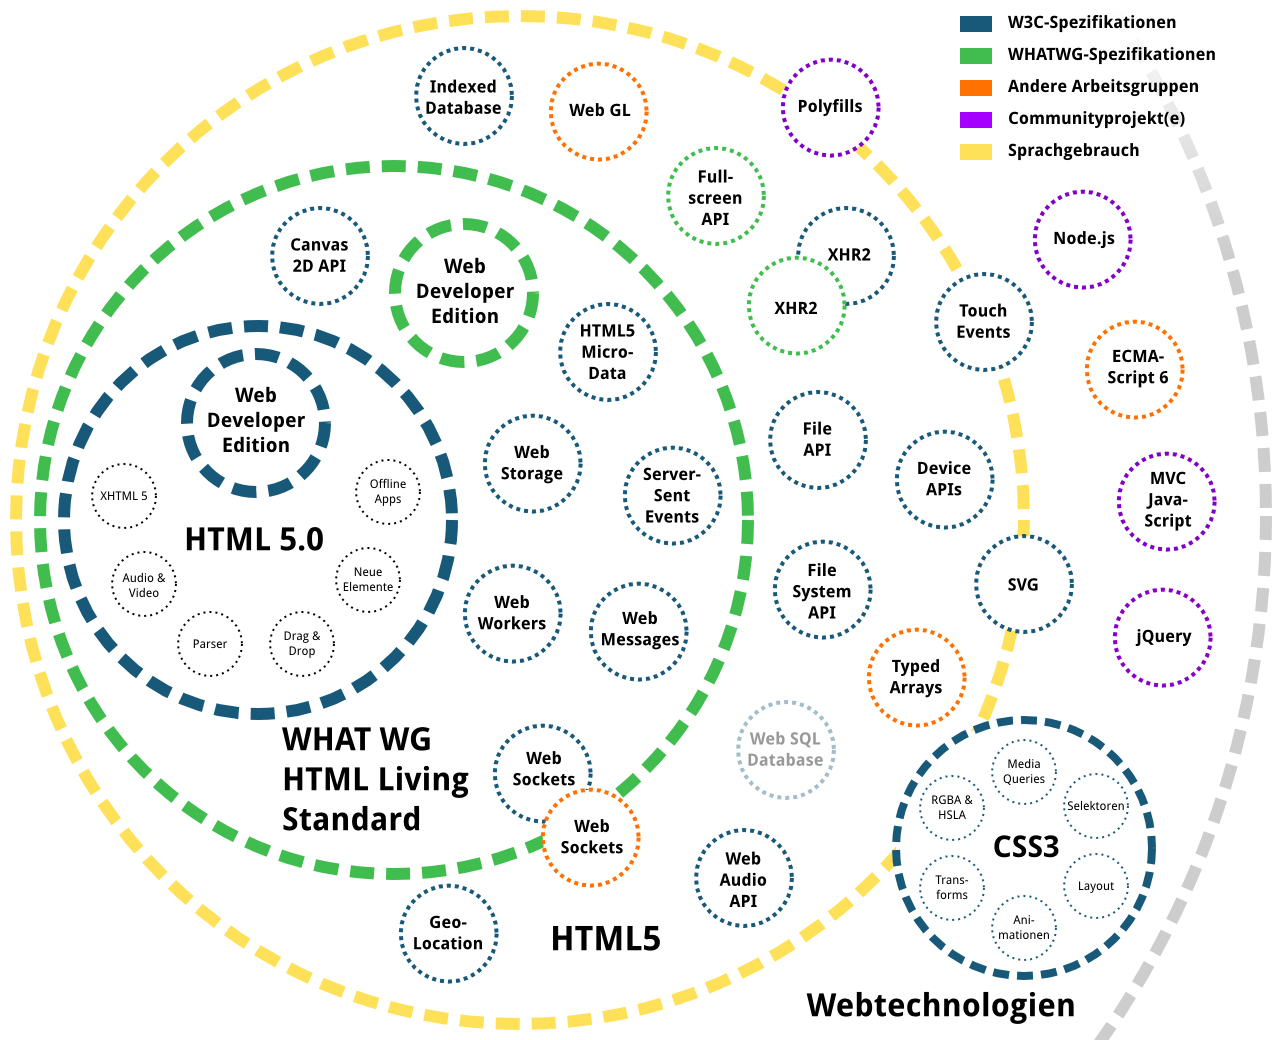
\includegraphics[width=0.87\linewidth]{images/html5_specs.png}
		\captionof{figure}[HTML5 Spezifikationen Übersicht]{HTML5 Spezifikationen Übersicht\cite{PeteKroe2014}}
		\label{fig:html5specs}
	\end{minipage}

\paragraph{Ziele} \ac{HTML}5 wurde mit besonderem Augenmerk auf die Kompatibilität entwickelt. Vorhandene Spezifikationen wie \ac{HTML} 4.01, \ac{XHTML} 1.0 und \ac{DOM} 2 sollten unter einem Dach gebündelt werden. Hierdurch wird der vorangegangenen Fragmentierung entgegen gewirkt. Schon vorhandene Inhalte müssen weitestgehend unterstützt werden auch wenn sie nicht zur \ac{HTML}5 Spezifikation gehören. Beispielsweise werden fehlerhaft verschachtelte Elemente trotzdem akzeptiert. \textit{Graceful degradation} ist als ein weiteres Ziel für HTML 5 definiert worden und bedeutet soviel wie \glqq Schrittweise Abstufung\grqq{}. Es stellt sicher, dass ein HTML Dokument auch dann verarbeitet wird sollte der verwendete Browser ein bestimmtes benutztes Element nicht unterstützen. Weiter galt für die Spezifikation, dass schon vorhandene Techniken, die weitläufig verbreitet sind, nicht neu entwickelt werden sollten. Stattdessen sollten sie übernommen werden. Dies beruht auf dem Umstand, dass die Browser Hersteller jeweils ihre eigenen Techniken bevorzugen und weiter entwickeln und dadurch auch für ihre Verbreitung sorgen. Evolution statt Revolution stand über den Zielen von HTML 5. (X)HTML wurde weiter entwickelt und nicht von Grund auf neu definiert. So ist in Tabelle \ref{tab:html5browserkomp} die zum aktuellen Zeitpunkt verfügbare Unterstützung von HTML 5 in den gängigsten Browsern abzulesen.

\vspace{1em}
\begin{table}[!h]
	\centering
	\begin{tabular}{|l|l|c|}
		\hline
		\textbf{Hersteller} & \textbf{Desktop/Mobile} & \textbf{Version}\\
		\hline
		Mozilla & Firefox & 4.0\\
		\hline
		 & Firefox Mobile & 16\\
		\hline
		Google & Chrome & 10\\
		\hline
		 & Chrome Mobile & 25\\
		\hline
		 & Android & 4.0\\
		\hline
		Apple & Safari & 5.1\\
		\hline
		 & Safari iOS & 5.1\\
		\hline
		Microsoft & Internet Explorer & 10\\
		\hline
		 & Windows Phone & 8\\
		\hline
		Opera Software & Opera & 11.64\\
		\hline
		Blackberry & Browser & 10\\
		\hline
	\end{tabular}
	\caption{HTML5 Browserkompatibilität}
	\label{tab:html5browserkomp}
\end{table}

\paragraph{Aufbau} Ein jedes HTML Dokument beginnt mit dem sogenannten \textit{Doctype}. Dieser legt fest mit welcher Syntax das Dokument aufgebaut ist und wie das Dokument vom Browser verarbeitet werden soll. Verschiedene Varianten wie \textit{strict},\textit{transitional} und \textit{frameset} sind in HTML5 nicht vorgesehen. In den Vorgängerversionen musste die Variante jedoch mit angegeben werden um eine eindeutige Interpretation des Dokuments zu gewährleisten. Listing \ref{lst:html401doctype} zeigt die beiden \textit{Doctype} von HTML 4.01 und XHTML 1.0. Durch die Abwärtskompatibilität von HTML5 sind auch diese \textit{Doctype} heute noch gültig und das Dokument wird korrekt vom Parser interpretiert werden.
    
    \vspace{1em}
	\begin{lstlisting}[caption=(X)HTML4.01 \textit{doctype}-Element, label=lst:html401doctype]
<!DOCTYPE HTML PUBLIC "-//W3C//DTD HTML 4.01//EN"
        "http://www.w3.org/TR/html4/strict.dtd">
<!DOCTYPE HTML PUBLIC "-//W3C//DTD HTML 4.01 Transitional//EN"
        "http://www.w3.org/TR/html4/loose.dtd">
<!DOCTYPE HTML PUBLIC "-//W3C//DTD HTML 4.01 Frameset//EN"
        "http://www.w3.org/TR/html4/frameset.dtd">        
<!DOCTYPE html PUBLIC "-//W3C//DTD XHTML 1.0 Strict//EN"
        "http://www.w3.org/TR/xhtml1/DTD/xhtml1-strict.dtd">    
	\end{lstlisting}
	
Listing \ref{lst:html5doctype}	hingegen zeigt das \textit{Doctype} von HTML5. Es wurde enorm gekürzt im Vergleich zu dem \textit{Doctype} von HTML 4.01 und XHTML 1.0. Groß- und Kleinschreibung ist nicht von bedeutung innerhalb des \textit{Doctype}. 

    \vspace{1em}
	\begin{lstlisting}[caption=HTML5 \textit{doctype}-Element, label=lst:html5doctype]
<!DOCTYPE html>
	\end{lstlisting}		
	
Nach dem \textit{Doctype} folgt der restliche Dokument Aufbau in HTML Syntax. Diese teilt sich auf in Elemente und Attribute, die diesen Elementen zugeordnet und mit Werten versehen werden können. Es existieren für die meisten Elemente Start- und Endmarkierungen. Für einige Elemente sind die Start- bzw. Endmarkierungen optional und für einige wiederum verpflichtend in der Dokumentstruktur zu setzen. In Listing \ref{lst:html5basicdoc} sieht man ein valides HTML5 Dokument mit den Mindestanforderungen.(vgl. \cite[S.58]{KronHTML2011})

	\vspace{1em}
	\begin{lstlisting}[caption=HTML5 Basis Dokument, label=lst:html5basicdoc]
<!DOCTYPE html>
<html>
 <head>
  <title>Beispiel Seite</title>
 </head>
 <body>
  <h1>Beispiel Seite</h1>
  <p>Dies ist ein <a href="demo.html">einfaches</a> Beispiel.</p>
  <!-- Dies ist ein Kommentar -->
 </body>
</html>
	\end{lstlisting}
	
\paragraph{Wichtige neue Sprachelemente} In HTML5 wurden die Mikrodaten mit aufgenommen. Mit Mikrodaten bietet sich eine weitere Möglichkeit ein HTML Dokument semantisch zu spezifizieren. Metadaten wie z.B. der verwendete Zeichensatz lassen sich so festlegen. Browser und Webseiten können über die Mikrodaten-\ac{API} die gesetzten Werte auslesen und weiter verarbeiten. Auch Suchmaschinen können auf die Metadaten zugreifen, verwenden sie jedoch heutzutage weitestgehend nicht mehr. Aus diesem Grund tragen die Metadaten zwar zur semantischen Struktur des HTML bei, können aber aus Sicht der Suchmaschinenoptimierung getrost vernachlässigt werden.(vgl. \cite{SelfHtml20142}) Weiter kann man bei Mikrodaten davon sprechen, \glqq [...] dass sie auf Name/Werte-Paaren basieren. Jedes Mikordatenvokabular definiert eine Menge benannter Eigenschaften.\grqq{}(vgl. \cite[S.174]{PilgDurc2011}) Listing \ref{lst:html5meta} zeigt Beispielhaft das \textit{head}-Element eines HTML Dokuments mit vier, darin eingeschlossenen, \textit{meta}-Elementen. Unter anderem wird mit dem ersten \textit{meta}-Element der Zeichensatz näher definiert. Das \textit{meta}-Element mit Namen \textit{viewport}, dient dazu die Skalierung auf Mobilgeräten zu unterdrücken, damit die Seite sich an den \textit{viewport} anpasst.

    \vspace{1em}
	\begin{lstlisting}[caption=HTML5 \textit{meta}-Element, label=lst:html5meta]
<head>
  <meta charset="utf-8">
  <meta name="viewport" content="width=device-width;" />
  <meta name="keywords" content="Lorem ipsum">
  <meta name="author"   content="dolor sem it">
</head>
	\end{lstlisting}
		
Zwei weitere neue Elemente in HTML5 sind das \textit{header}- und \textit{footer}-Element. Zu Zeiten vor HTML5 wurden jene Bereiche einer Website durch \textit{div}-Elemente mit dem \textit{id}- oder \textit{class}-Attribut entsprechend gekennzeichnet. Das ist jetzt nicht mehr nötig durch die beiden neuen Elemente. Üblich ist es im \textit{header}-Element einer Website Komponenten wie das Logo, das Menü und den Titel unterzubringen. Im \textit{footer}-Element dagegen werden Kontakt, Impressum und das Copyright aufgeführt. In Listing \ref{lst:html5header}	 ist die Platzierung des \textit{header}- und \textit{footer}-Elements innerhalb eines \textit{body}-Elements einer Webseite zu sehen.

    \vspace{1em}
	\begin{lstlisting}[caption=HTML5 \textit{header}- und \textit{footer}-Element, label=lst:html5header]
<body>
  <header>
    <img src="logo.gif" alt="logo">
    <h1>Ueberschrift</h1>
  </header>
  <footer>
     <a href="kontakt.html">Kontakt</a>
  </footer>
</body>
	\end{lstlisting}
	
Um ein HTML Dokument nach heutigen Maßstäben korrekt zu strukturieren wurden einige Elemente der Spezifikation hinzugefügt. So lässt sich die Navigation nun mit dem \textit{nav}-Element umschließen wie in Listing \ref{lst:html5struct} ab Zeile 3 zu sehen. \glqq Das \textit{section}-Element repräsentiert einen allgemeinen Abschnitt in einem Dokument oder einer Anwendung. Ein Abschnitt ist in diesem Kontext eine thematische Gruppierung von Inhalten, die üblicherweise unter einer Überschrift stehen. Beispiele für Abschnitte wären Kapitel, die verschiedene Tabs in einem Dialog mit Tabs oder die nummerierten Abschnitte einer wissenschaftlichen Arbeit.[...] Das \textit{article}-Element repräsentiert eine abgeschlossene Einheit in einem Dokument, einer Anwendung oder einer Site, die unabhängig verbreitet oder wiederverwendet werden kann, z.B. in RSS-Feeds. Es könnte beispielsweise ein Forenbeitrag, ein Zeitschriften- oder Zeitungsartikel, ein Blog-Eintrag, ein Benutzerkommentar, ein interaktives Widget oder Gadget oder ein Element mit unabhängigem Inhalt enthalten. Das \textit{aside}-Element repräsentiert einen Abschnitt einer Seite, der Inhalte enthält, die sich zwar auf den das \textit{aside}-Element umgebenden eigentlichen Inhalt der Seite beziehen, aber als von ihm unabhängig betrachtet werden können. In Druckwerken werden derartige Abschnitte häufig als Seitenleisten dargestellt. Das Element kann für typografische Effekte wie herausgehobene Zitate oder Seitenleisten, für Werbung, für Gruppen von \textit{nav}-Elementen und andere Inhalte verwendet werden, die als vom eigentlichen Inhalt der Seite getrennt betrachtet werden können.\grqq{}\cite[S.43]{PilgDurc2011} Das neue \textit{main}-Element ist zur Auszeichnung des Seitenhauptinhalts vorgesehen. Mit dieser Auszeichnung lässt sich z.B. mit Screenreadern direkt zum Hauptinhalt springen.  Alle genannten Elemente sind in Listing \ref{lst:html5struct} in ihrer vorgesehenen Reihenfolge abgebildet.

    \vspace{1em}
	\begin{lstlisting}[caption=HTML5 Struktur Elemente, label=lst:html5struct]
<body>
  <header>
    <nav>
      <ul>
        <li><a href="#link_1.html">Wiki</a></li>
        ...
      </ul>
    </nav>
  </header>
  <main>
  <article>
    <h1>Ueberschrift</h1>
    <p>Dies ist eine Beispiel HTML5-Seite</p>
  </article>
  <aside>
    <section>
      <h2>Kontakt</h2>
      <ul>
        <li><a href="link_1.html">Wiki</a></li>
        ...
      </ul>
    </section>
  </aside>
  </main>
  <footer>
  </footer>
</body>
	\end{lstlisting}

\glqq Damit auch ältere Internet Explorer der Versionen 6-8 die neuen HTML5-Elemente darstellen können, kann ein kurzes JavaScript eingebunden werden. Am einfachsten ist es, dieses nicht auf dem eigenen Server vor zuhalten, sondern direkt von Google abzurufen. Dies hat überdies den Vorteil, dass es oft schon im Browser-Cache der Nutzer vorhanden ist. Der Aufruf erfolgt in einem \textit{Conditional Comment}, der nur vom Internet Explorer kleiner als Version 9 (lt IE 9) verstanden wird. Alle andere Browser ignorieren dies als reinen Kommentar.\grqq{}\cite{SelfHtml20143} In Listing \ref{lst:html5fallback}	 ist der beschriebene Rückfallmechanismus verdeutlicht.

    \vspace{1em}
	\begin{lstlisting}[caption=HTML5 Internet Explorer Fallback, label=lst:html5fallback]
<head>
  <meta charset="utf-8">
  <!--[if lt IE 9]>
    <script src="//html5shim.googlecode.com/svn/trunk/html5.js"></script>
  <![endif]-->
  <title>HTML5-Seite mit Grundstruktur</title>
</head>
	\end{lstlisting}
	
Eingabefelder sind in den meisten Applikationen unabdingbar. Aus diesem Grund wurden in HTML5 eine vielzahl an \textit{input}-Elementen hinzugefügt. So müssen keine komplizierten Workarounds mit JavaScript oder anderen Skriptsprachen mehr verwendet werden. \glqq Das typische HTML5-Formular unterscheidet sich nicht fundamental von seinen in HTML 4.01 oder XHTML 1 geschriebenen Gegenstücken. Alle alten Formularelemente sind noch da und verhalten sich weitgehend wie bisher. Die Neuerungen bestehen aus einigen neuen Funktionen, Attributen und \ac{API}s und aus einer ganzen Reihe neuer möglicher Werte für das \textit{type}-Attribut des \textit{input}-Elements.\grqq{}\cite[S.176]{KronHTML2011} In Listing \ref{lst:html5input} sind beispielhaft einige neue Werte des \textit{type}-Attributs ausgeführt. Eingabefelder des Typs \textit{tel, email} oder \textit{url} sind vom Verständnis her simple Texteingabefelder. Als wichtige Besonderheit lässt sich bei \textit{email}- und \textit{url}-Feldern aber ihre eingebaute Validation nennen. Verwendet man die Validierungs-\ac{API} werden nur korrekte URLs bzw. E-Mails zugelassen. Für ein \textit{tel}-Feld gilt dies nicht. Außerdem wird auf Smartphones und Tablet-Geräten die angezeigte Bildschirmtastatur entsprechend des erwarteten Eingabetyps für eine optimale Eingabe angepasst dargestellt.(vgl. \cite[S.178]{KronHTML2011}) So wird bei einer erwarteten E-Mail Adresse das @-Symbol direkt auf der Bildschirmtastatur als eigene Taste mit angezeigt, was normalerweise nicht der Fall ist. Einige der neuen Elementausprägungen besitzen noch zusätzliche Attribute die die Eingabemöglichkeit weiter einschränken und präzisieren können. Zu sehen in Zeile 5 von Listing \ref{lst:html5input} im \textit{time}-Feld, bei dem die erwartete Zeit von 9:00Uhr bis 17:00Uhr nur einstellbar ist. \textit{input}-Elemente können über das \textit{required}-Attribut außerdem als Pflichtfeld markiert werden.

    \vspace{1em}
	\begin{lstlisting}[caption=HTML5 \textit{input}-Element, label=lst:html5input]
<body>
  <input type="tel">
  <input type="email">
  <input type="url">  
  <input type="time"  min="09:00" max="17:00">
  <input type="date"  required="required">
</body>
	\end{lstlisting}
	
Für multimediale Inhalte auf Webseiten wurden der Spezifikation passende Elemente hinzugefügt. Das \textit{canvas}-Element \glqq [...] stellt eine Fläche zur Verfügung, auf die mittels JavaScript dynamische Bitmap-Grafiken gezeichnet werden können. So lassen sich Animationen erstellen, Diagramme zeichnen, eigene Interface-Elemente kreieren und Videos manipulieren\grqq{}\cite[S.353]{KronHTML2011} Für Audio und Video Inhalte wurden die gleichnamigen Elemente geschaffen. 
	
\subsection{CSS3}
\glqq Cascading Style Sheets (CSS) bieten mächtige Möglichkeiten, die Präsentation eines Dokuments oder einer Sammlung von Dokumenten zu beeinflussen. Offensichtlich ist CSS ohne irgendein Dokument ziemlich nutzlos, da es keine Inhalte zu präsentieren gäbe.\grqq{}\cite[S.1]{MeyeCasc2005} CSS gehört mit zu den Kernsprachen des WWW. \glqq Zuallererst ermöglicht CSS eine wesentlich umfangreichere Gestaltung des Aussehens eines Dokuments, als HTML das jemals konnte, nicht einmal als die Präsentationselemente einen Großteil der Sprache ausmachten. Mit CSS kann für jedes Element eine eigene Text- und Hintergrundfarbe festgelegt werden. Jedes Element lässt sich zudem mit einem Rahmen versehen; der Platz um ein Element herum kann in der Größe verändert werden und es kann Einfluss auf die Groß- und Kleinschreibung genommen werden. Mit CSS können Sie außerdem  bestimmen, wie fett bestimmte Textteile dargestellt werden sollen, welche Dekoration (z.B. Unterstreichungen) verwendet werden soll, wie groß die Abstände zwischen einzelnen Buchstaben und Wörtern sein sollen und ob der Text überhaupt angezeigt wird.\grqq{}\cite[S.4]{MeyeCasc2005} Mit CSS ist es möglich das Aussehen der Webseite mit Bezug auf das verwendete Anzeigegerät anzupassen und entsprechend optimiert darzustellen.

\paragraph{Einbindung} Um eine Webseite überhaupt mit CSS zu gestalten muss es innerhalb eines HTML Dokuments eingebunden sein. Dies ist auf drei verschiedene Arten möglich. Als Erstes mal das \textit{link}-Element. \glqq CSS benutzt dieses Tag, um Stylesheets mit dem Dokument zu verbinden.[...] Stylesheets, die nicht im HTML-Dokument selbst enthalten sind, sondern von außen eingebunden werden, bezeichnet man als externe Stylesheets[...].Um ein Stylesheet erfolgreich zu laden, muss sich ein \textit{link} innerhalb des \textit{head}-Elements befinden, darf aber nicht innerhalb eines anderen Elements wie etwa \textit{title} stehen.\grqq{}\cite[S.14]{MeyeCasc2005} In Listing \ref{lst:css3einbindunglink} ist die Einbindung eines externen Stylesheets über das \textit{link}-Element zu sehen.
	
	\vspace{1em}
	\begin{lstlisting}[caption=Stylesheet Einbindung über \textit{link}-Element, label=lst:css3einbindunglink]
<head>
    <link rel="stylesheet" type="text/css" href="beispiel.css" />
</head>
	\end{lstlisting}

Eine andere Möglichkeit ist es das CSS direkt innerhalb eines \textit{style}-Elements zu positionieren. Ein Element vom Typ \glqq \textit{style} sollte immer zusammen mit dem Attribut \textit{type} verwendet werden. Im Fall eines eingebetteten CSS-Dokuments ist der korrekte Wert \glqq \textit{text/css}\grqq, genau wie bei dem Element \textit{link}.[...] Die Stildefinition zwischen den öffnenden und schließenden \textit{style}-Tags bezeichnet man als Dokumenten-Stylesheet oder auch als eingebettetes Stylesheet[...].\grqq{}\cite[S.19]{MeyeCasc2005} Listing \ref{lst:css3einbindungstyle} zeigt ein solches eingebettetes Stylesheet.

	\vspace{1em}
	\begin{lstlisting}[caption=Stylesheet Einbindung über \textit{style}-Element, label=lst:css3einbindungstyle]
<head>
	<title>Dokument mit Formatierungen</title>
	<style type="text/css">
		body { color: purple; background-color: #d8da3d; }
	</style>
</head>
	\end{lstlisting}
	
Als letzte Möglichkeit kann man ein Stylesheet bzw Style-Informationen direkt einem HTML Element anhängen. \glqq Durch das direkte Festlegen von Formaten, umgangsprachlich auch \glqq Inline-Style\grqq{} genannt, gehen viele Vorteile verloren. Der Wartungsaufwand steigt während die Flexibilität sich verringert. Inline-Styles sind an ein Dokument gebunden und können nicht an zentraler Stelle bearbeitet werden.\grqq{}\cite{SelfHtml20144} In Listing \ref{lst:css3einbindunghtml} wird dem \textit{span}-Element ein \glqq Inline-Style\grqq gegeben.

	\vspace{1em}
	\begin{lstlisting}[caption=Stylesheet Einbindung in \textit{html}-Element, label=lst:css3einbindunghtml]
<span style="font-size: small;">Text</span>
	\end{lstlisting}
	
Innerhalb von CSS-Dateien kann man wiederum mit der Direktive \textit{@import} den Browser dazu zu bringen weitere Stylesheets nachzuladen und zu verwenden. Zu beachten ist, dass die \textit{@import} Direktive vor allen anderen CSS Befehlen steht, bei den eingebetteten wie auch den externen Stylesheets.(vgl. \cite[S.20]{MeyeCasc2005})

\paragraph{Syntax} Die Syntax von CSS ist denkbar einfach. Sie besteht im wesentlichen aus dem Selektor und dem Deklarationsblock. Ein Selektor entspricht in den häufigsten Fällen dem gleichnamigen HTML Element. Der Deklarationsblock wiederum besteht aus mindestens einer Deklaration.(vgl. \cite[S.26]{MeyeCasc2005}) \glqq Eine Deklaration besteht dabei immer aus einer Eigenschaft, die mit einem Wert durch einen Doppelpunkt verbunden ist. Abgeschlossen wird die Deklaration durch ein nachgestelltes Semikolon. Auf den Doppelpunkt und das Semikolon kann eine beliebige Anzahl von Leerzeichen (also auch keines) folgen. Fast immer besteht der Wert aus einem einzelnen Schlüsselwort oder einer durch Leerzeichen getrennten Liste aus mehreren Schlüsselwörtern, die für die genannte Eigenschaft zulässig sind.\grqq{}\cite[S.28]{MeyeCasc2005} Verwendet man in der Deklaration ungültige Eigenschaften oder Werte werden diese einfach ignoriert. Listing \ref{lst:css3syntax} zeigt die Syntax beispielhaft.

	\vspace{1em}
	\begin{lstlisting}[caption=CSS3 Syntax Beispiel, label=lst:css3syntax]
Selektor [, Selektor2, ...] {
    Eigenschaft1: Wert1;
    ...
    EigenschaftN: WertN[;]
}
	\end{lstlisting}

Um sich wiederholende Design Regeln zusammenfassen zu können lassen sich Selektoren in CSS gruppieren. Dabei werden die zu gruppierenden Selektoren durch ein Komma von einander getrennt und dann die zu gestaltenden Eigenschaften mit den entsprechenden Werten genannt wie in Listing \ref{lst:css3group} zu sehen.

	\vspace{1em}
	\begin{lstlisting}[caption=CSS3 Gruppierung, label=lst:css3group]
h1, h2, p {
  color: black;
}
	\end{lstlisting}

\paragraph{Selektoren} CSS arbeitet wie HTML auch mit dem \ac{DOM}. \glqq Der erste Vorteil, der sich aus dem Verständnis dieses Modells ergibt, ist die Möglichkeit, Selektoren für Nachfahren (auch als Kontext-Selektoren bezeichnet) zu definieren. Die Definition von Selektoren für Nachfahren besteht aus dem Festlegen von Regeln, die nur für bestimmte hierarchische Strukturen gelten.\grqq{}\cite[S.48]{MeyeCasc2005} Der erst genannte Selektor ist das Elternelement. Mittels eines Leerzeichens wird das Nachfahren Element vom Elternelement getrennt. In Listing \ref{lst:css3kids} wird angegeben, dass jedes \textit{strong}-Element innerhalb eines \textit{h1}-Elements eine besondere Formatierung erhält. Konkret bedeutet das in diesem Fall, dass die Schriftgröße 14pt und die Schriftgewichtung, welche die Dicke und Stärke festlegt, \textit{bold} sein soll. Zu beachten ist, dass so sämtliche Nachfahren des \textit{h1}-Elements entsprechend formatiert werden. Es gibt auch die Möglichkeit die Formatierung nur auf einen direkt Nachfahren, ein sogenanntes Kindelement, zu beschränken. Um dies zu erreichen werden Eltern- und Kindelement nicht durch ein Leerzeichen von einander getrennt, sondern durch das Größer-als-Zeichen (\textgreater).

	\vspace{1em}
	\begin{lstlisting}[caption=CSS3 Selektoren für Nachfahren, label=lst:css3kids]
h1 strong {
  font-size:  14pt;
  font-weight: bold;  
}
	\end{lstlisting}

Das gleiche Verfahren kann auch auf Nachbarelemente angewandt werden. Nur wird hierbei ein anderes Kombinatorenzeichen benötigt, nämlich das Plus (+).\\
\glqq Zusätzlich zu den rohen Dokument-Elementen gibt es noch zwei weitere Arten von Selektoren: Klassenselektoren und ID-Selektoren, mit denen sich Stildefinitionen unabhhängig von den Elementen eines Dokuments zuweisen lassen. Diese Selektoren können eigenständig oder zusammen mit Elementselektoren verwendet werden. Allerdings ist es hierfür notwendig, die Dokumentteile entsprechend zu markieren. Die Benutzung dieser neuen Selektoren erfordert daher [...] Voraussicht und Planung.\grqq{}\cite[S.34ff]{MeyeCasc2005} Des weiteren muss die HTML Auszeichnung angepasst werden sollten Klassen- und/oder ID-Selektoren verwendet werden. Konkret bedeutet dies, dass jedem HTML Element ein \textit{class}- und/oder \textit{id}-Attribut hinzugefügt werden muss sofern es von den CSS Regeln beachtet werden soll. Zu beachten ist, dass eine vergebene ID im gesamten HTML Dokument einzigartig sein muss, wohingegen eine vergebene Klasse auf mehrere HTML Elemente und auf ein HTML Element auch mehrere Klassen angewandt werden können. (vgl. \cite{W3ScCss2014}) Listing \ref{lst:css3idclass} zeigt einen solchen ID-Selektor, einen Klassenselektor und einen Klassenselektor der nur auf \textit{p}-Elementen gilt die das \textit{class}-Attribut besitzen.

	\vspace{1em}
	\begin{lstlisting}[caption=CSS3 Klassen- und ID-Selektoren, label=lst:css3idclass]
<div id="ID">
  <p class="Klasse"></p>
</div>

div#ID {
  text-align: center;
  color:      red;
}
.Klasse {
  text-align: center;
  color:      red;
}
p.Klasse {
  text-align: center;
  color:      red;
}
	\end{lstlisting}
	
\paragraph{Pseudoklassen} Neben den genannten gibt es noch einen weiteren Typ von Selektoren. Die sogenannten Pseudoselektoren für die Pseudoklassen. \glqq Mit diesen Selektoren [... kann man] Stildefinitionen auf Strukturen zuweisen, die nicht unbedingt im Dokument vorkommen müssen, oder auch [... Pseudo]klassen, die vom Zustand bestimmter Elemente oder sogar vom Zustand des Dokuments selbst abhängen. Anders gesagt, werden die Stile, basierend auf etwas anderem als der Struktur des Dokuments, auf Teile des Dokuments angewendet.\grqq{}\cite[S.53ff]{MeyeCasc2005} Um beispielsweise einen Link in einem Dokument farblich zu markieren sobald er besucht wurde wäre eigentlich für jeden Zustand des Links eine eigene Klasse nötig. Diese Klasse müsste sich ständig ändern je nach dem ob der Nutzer den Link schon besucht hat oder nicht. Um diesen Umstand zu verhindern existieren die Pseudoselektoren und Pseudoklassen. Im Fall eines \textit{a}-Elements werden die Pseudoklassen \textit{link} und \textit{visited} bereitgestellt um den Effekt zu erzeugen. Diese Klassen werden dem \textit{a}-Element durch CSS selber hinzugefügt bzw. wird ein \textit{a}-Element, das ein \textit{href}-Attribut besitzt und noch nicht besucht wurde mit der Pseudoklasse \textit{link} versehen. Die Pseudoklasse \textit{visited} bezieht sich auf \textit{a}-Elemente mit \textit{href}-Attribut die schon besucht wurden. Listing \ref{lst:css3pseudo} zeigt ein solches \textit{a}-Element und die beiden Pseudoselektoren.

	\vspace{1em}
	\begin{lstlisting}[caption=CSS3 Pseudoklassen und -selektoren, label=lst:css3pseudo]
<a href="http://www.example.com">Example.com</a>

/* unvisited link */
a:link {
    color: #FF0000;
}

/* visited link */
a:visited {
    color: #00FF00;
}
	\end{lstlisting}

\paragraph{Box-Modell} \glqq CSS geht davon aus, dass jedes Element eine oder mehrere rechteckige Boxen erzeugt, die Element-Boxen genannt werden.[...] Im Kern besitzt jede Box einen Inhaltsbereich (content area). Dieser wird umgeben von optionalen Innenabständen (padding), Rahmen (borders) und Außenabständen (margins). Diese Teile werde als optional angesehen, weil sie alle eine Breite von null Einheiten haben können, also sozusagen nicht vorhanden sind.\grqq{}\cite[S.167]{MeyeCasc2005} \glqq Da eine Box aus mehreren Komponenten bestehen kann, werden für die einzelnen Bereiche verschiedene Kantenbezeichnungen definiert. Als Innen- oder Inhaltskante wird die Strecke bezeichnet, die den Inhaltsbereich einer Box umfasst. Das ist der Bereich, der durch den Inhalt oder die Eigenschaften \textit{width} und \textit{height} festgelegt wurde. Der Bereich einer Box, der von den Innenkanten umgeben ist, wird auch \textit{content box} (Inhaltsbox) genannt. Die Kanten, die eine Box mitsamt Innenabstand umfassen, werden Polsterungskanten genannt. Der von diesen Kanten umfasste Bereich wird \textit{padding box} (Polsterungsbox) genannt. Besitzt eine Seite keinen Innenabstand, so ist die Polsterungskante mit der Innenkante identisch. Die Rahmenkanten umgeben eine Box mit deren Rahmen. Der durch diese Kanten abgesteckte Bereich wird \textit{border box} (Rahmenbox) genannt. Besitzt eine Box keinen Rahmen, so ist die Rahmenkante mit der Polsterungskante identisch. Eine vollständige Box wird durch die Außenkanten definiert. Die Außenkante umfasst eine Box mitsamt Außenabständen, also die \textit{margin box}. Sind für eine Box keine Außenabstände definiert, so ist die Außenkante mit der Rahmenkante identisch.\grqq{}\cite{SelfHtml20145}\\Die Gesamtbreite eines Elements definiert sich dadurch als Summe aus Breite, linkem und rechtem Innenabstand, linkem und rechtem Rahmen und dem linkem und rechtem Außenabstand. Für die Gesamthöhe verhält sich die Berechnung analog. Abbildung \ref{fig:cssboxmodell} zeigt das beschriebene CSS-Box-Modell.

	\vspace{1em}
	\begin{minipage}{\linewidth}
		\centering
		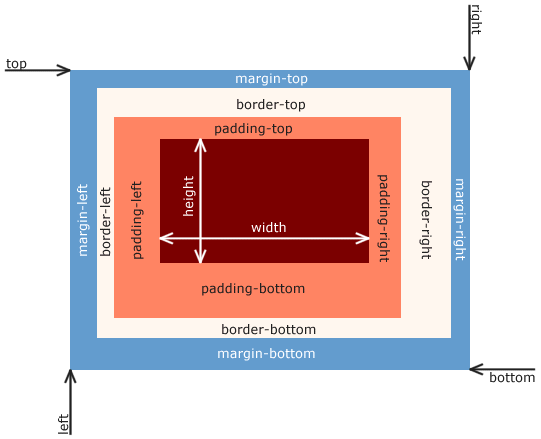
\includegraphics[width=0.8\linewidth]{images/css_boxmodell.png}
		\captionof{figure}[CSS-Boxmodell]{CSS-Box-Modell\cite{WikiCSS2014} }
		\label{fig:cssboxmodell}
	\end{minipage}
	
\paragraph{Spezifische Stylesheets} \glqq Dank der Mechanismen in CSS und HTML [... lassen sich] beliebige Stylesheets auf bestimmte Medien beschränken. In HTML-basierten Stylesheets geschieht dies mit Hilfe des Attributs \textit{media} und gilt sowohl für \textit{link}- wie auch \textit{style}-Elemente. Das Attribut \textit{media} akzeptiert entweder die Angabe eines einzelnen Mediums oder eine durch Komma getrennte Liste von Werten.\grqq{}\cite[S.434ff]{MeyeCasc2005} Die Angaben in Listing \ref{lst:css3media} bewirken eine gesonderte Formatierung für ein \textit{print} Medium.

	\vspace{1em}
	\begin{lstlisting}[caption=CSS3 medienspezifisches Stylesheet, label=lst:css3media]
<link rel="stylesheet" type="text/css" media="print" href="article-print.css">
	\end{lstlisting}
	
Ein vorhandenes Stylesheet ohne Medieninformationen gilt für alle Medien. Fernen lassen sich die Medien auch innerhalb des Stylesheets näher beschreiben durch den \textit{@media}-Block. Diesen \textit{@media}-Blöcken können neben den Medientypen auch noch weitere Bedingungen hinzugefügt werden. In Listing \ref{lst:css3mediaquery} wird das Element mit der ID \textit{inhalt} auf eine Breite von \textit{800px} festgelegt. Ist das verwendete Ausgabemedium jedoch ein Bildschirm und hat nur eine Gesamtbreite von \textit{1024px} wird das Element mit der ID \textit{inhalt} auf eine Breite von nur noch \textit{600px} und das \textit{aside}-Element gar nicht mehr angezeigt.

	\vspace{1em}
	\begin{lstlisting}[caption=CSS3 eigenschaftsspezifisches Stylesheet, label=lst:css3mediaquery]
#inhalt {
	width: 800px;
}
 
@media screen and (max-width: 1024px) {
	#inhalt {
		width: 600px;
	}
	aside {
		display: none;
	}
}
	\end{lstlisting}

\subsection{JavaScript}
\paragraph{Historie} JavaScript wurde 1995 von Netscape entwickelt, lizenziert und eingeführt. Um der Sprache von Anfang an einen Standardcharakter zu geben wurde die Organisation \ac{ECMA} hinzugezogen. Die ECMA veröffentlichte unter dem Namen ECMAScript einen, auf Netscapes JavaScript Spezifikation basierenden, Industriestandard der Sprache. Da JavaScript somit eine proprietäre Sprache von Netscape ist, hat Microsoft seine eigene Variante, mit Namen JScript, veröffentlicht. JScript implementiert JavaScript vollständig, besitzt allerdings auch noch Zusatzfunktionen wie z.B. Zugriff auf das Dateisystem und das Betriebssystem Windwos. Mit Version 1.5 von JavaScript erhielt das DOM Einzug in die Implementierung. Da jeder Browser seinen eigenen JavaScript Interpreter besaß, war es kaum Möglich einheitlichen Code für alle Browser zu entwickeln. Es musste auf alle Eventualitäten geachtet werden. Um diesem Missstand entgegen zu wirken wurde das W3C hinzugezogen um einen einheitlichen Sprachstandard zu etablieren. Jedoch entwickelte das W3C keinen konkreten JavaScript-Standard, sondern eine Schnittstelle - das erwähnte DOM. Die aktuelle JavaScript Version von 2010 ist 1.8.5 und ECMAScript liegt in Version 5.1 seit Juni 2011 vor. (vgl. \cite{SelfHtml20146})

\paragraph{Sandbox-Prinzip} JavaScript wird innerhalb eines Browser in einer sogenannten Sandbox ausgeführt. Das bedeutet es liegt in einem abgesichertem Speicherbereich, aus welchem es keinen Zugriff auf Objekte außerhalb des Browsern hat. Eine Ausnahme ist der Lesezugriff auf Dateien die mittels des \textit{input}-Elements von einem Nutzer selbst hoch geladen werden. Des weiteren kann mit JavaScript auch nicht ohne weiteres auf bestimmte sicherheitskritische Funktionen des ausführenden Browser zugegriffen werden. Um beispielsweise das Browserfenster zu schließen, Symbolleisten ein- und auszublenden oder zugriff auf die Seitenhistorie zu erlangen sind Nutzereingaben nötig. (vgl. \cite{WikiJS2014})

\paragraph{Objektorientierung} \glqq JavaScript gehört zu den sogenannten objektorientierten Programmiersprachen (oder, um genauer zu sein, zu den objektbasierten Sprachen). Das Konzept der objektorientierten Programmierung (OOP) wird im Folgenden sehr stark vereinfacht erklärt.[...] In JavaScript ist (mit Ausnahme der Variablen) alles, worauf man zugreift, ein Objekt. Ein Objekt ist der Versuch, die reale Welt in eine Programmiersprachenumgebung abzubilden. Ein Standardbeispiel für Objekte ist etwa ein Auto. Das Auto an sich (als abstrakter Begriff) kann als Objekt angesehen werden, ein einzelnes Auto wird als Instanz des Objekts Auto bezeichnet.\grqq{}\cite[S.93]{WenzJava2008} Ein Auto bzw. ein Objekt generell lässt sich durch Parameter näher beschreiben. Diese Parameter gibt es in zwei Ausführungen. Die Eigenschaften und die Methoden. Bei einer Eigenschaft handelt es sich im Grunde um eine Variable die einen festen Bezug zum Objekt besitzt. Eigenschaften können gelesen und gesetzt werden. Ein Auto hat beispielsweise als Eigenschaft die Anzahl der Türen oder die Motorleistung. Methoden auf der anderen Seite müssen nicht immer einen Informationswert zurückgeben. Bei dem Objekt Auto könnte es eine Methode \textit{tunen()} geben die dann Einfluss auf die Eigenschaft Motorleistung nimmt.\\Im Kontext der Webentwicklung mit JavaScript existieren einige feste Objekte die zu jederzeit zur Verfügung stehen. Da wäre zum einen das \textit{window}-Objekt, dass, wie der Name schon erahnen lässt, das aktuelle Browserfenster repräsentiert. Über die Eigenschaften und Methoden lassen sich Informationen zum Browserfenster erhalten und beispielsweise neue Fenster öffnen. Das \textit{document}-Objekt bildet den Inhalt eines Browserfensters ab. Es stellt das Ausgangsobjekt für das DOM dar. Es steht in der Hierarchie direkt unter dem \textit{window}-Objekt. Neben diesen Objekten existieren noch weitere um den Browserkontext möglichst genau innerhalb einer JavaScript Anwendung verfügbar zu machen.(vgl. \cite{SelfHtml20147})

\paragraph{Sprachelemente} JavaScript wird mit dem Unicode Zeichensatz geschrieben. Die 16-Bit-Codierung bei Unicode enthält fast sämtliche Zeichen der Schriftsprachen der Welt. Die Nutzung von Unicode trägt wesentlich zu der Internationalisierung bei. Bei der Groß- und Kleinschreibung unterscheidet JavaScript eindeutig. So müssen alle Schlüsselwörter und Bezeichner immer in der selben vorgegebenen Schreibweise geschrieben werden, damit sie vom JavaScript Interpreter korrekt behandelt werden. Whitespace, Tabulatoren und Zeilentrenner werden vom Interpreter komplett ignoriert und können deshalb zur visuellen Strukturierung des Programmcodes genutzt werden. Dadurch kann der Programmcode leicht leserlich und verständlich formatiert werden ohne das dadurch die Logik verletzt wird. Das, aus anderen Programmiersprachen bekannte, Semikolon am Ende einer Anweisung ist in JavaScript nicht zwingend erforderlich. Eine Anweisung ist im Normalfall mit dem Ende der Zeile abgeschlossen. So muss ein Semikolon lediglich gesetzt werden, wenn sich mehr als eine Anweisung in der Zeile befinden oder eine Anweisung über mehrere Zeilen hinweg formuliert wurde. Fehlende Semikola werden vom Interpreter selbst gesetzt, was in bestimmten Fällen aber zum Bruch der Logik führen kann wie in Listing \ref{lst:jssemikolon} zu sehen.(vgl. \cite[S.15ff]{FlanJava2007})

	\vspace{1em}
	\begin{lstlisting}[caption=JavaScript Logikbruch Semikolon, label=lst:jssemikolon]
// kein Interpretierungsfehler
a = 3
b = 4;

// korrekte Schreibweise in einer Zeile
a = 3; b = 4;

// Interpreter setzt Semikolon automatisch
return
true;
// falsche Interpretation anschliessend
return;
true;
	\end{lstlisting}

Des weiteren gibt es einige Literale in JavaScript. \glqq Ein Literal ist ein Datenwert, der direkt in einem Programm vorkommt. Literale können zum Beispiel folgendermaßen aussehen:\grqq{}\cite[S.18]{FlanJava2007}

	\vspace{1em}
	\begin{lstlisting}[caption=JavaScript Literale, label=lst:jsliterale]
12                // Die Zahl zwoelf
1.2               // Die Zahl eins komma zwei
"Hallo Welt"      // Ein Text-String
'Hi'              // Noch ein String
true              // Ein Boolescher Wert
false             // Der andere Boolesche Wert
null              // Kein Objekt vorhanden
	\end{lstlisting}
	
Im offiziellen Standard ECMAScript existieren außerdem Literale, die zur Initialisierung von Arrays und Objekten dienen. Neben den genannten Sprachelementen gibt es noch die Bezeichner. Ein Bezeichner ist ein Name in JavaScript. Er dient dazu Variablen, Funktionen und einige Schleifen-Marker zu benennen. Ein Bezeichner unterliegt gewissen Regeln. Zum einen muss das erste Zeichen ein Buchstabe, ein Unterstrich (\_) oder ein Dollar-Zeichen (\$) sein. Der restliche Bezeichner darf aus Buchstaben, Ziffern, Unterstrichen oder Dollar-Zeichen bestehen. Eine weitere Regel legt fest, dass ein Bezeichner nicht wie ein Schlüsselwort heißen darf. Tabelle \ref{tab:jskeywords} listet die Schlüsselwörter von JavaScript auf.(vgl. \cite[S.19]{FlanJava2007})

\vspace{1em}
\begin{table}[!h]
	\centering
	\begin{tabular}{|l|l|l|l|l|}
		\hline
		break & do & if & switch & typeof\\
		\hline
		case & else & in & this & var\\
		\hline
		catch & false & instanceof & thorw & void\\
		\hline
		continue & finally & new & true & while\\
		\hline
		default & for & null & try & with\\
		\hline
		delete & function & return & &\\
		\hline
	\end{tabular}
	\caption{JavaScript Schlüsselwörter}
	\label{tab:jskeywords}
\end{table}

\paragraph{Datentypen und Werte} Werte zur Berechnung werden in Variablen mit bestimmten Datentypen gesichert. Dazu unterstützt JavaScript einige primitive Datentypen wie Zahlen, Text und boolesche Werte. Außerdem gibt es einen zusammengesetzten Datentypen, das Objekt, mit dem eine Sammlung von verschiedenen Werten dargestellt wird. So kann ein Objekt beispielsweise auch weitere Objekte beinhaltet. Sind die Werte in geordneter nummerierter Reihenfolge nennt man das Objekt Array. Die Zahlen sind der einfachste Datentyp. Mit ihm werden Zahlen dargestellt, egal ob Ganzzahlig oder Gleitkommazahlen. JavaScript behandelt jede Zahl als Gleitkommazahl und stellt diese im 64-Bit-Gleitkommaformat nach IEEE 754 dar.\\Integer-Literale werden in JavaScript als eine Folge von Ziffern geschrieben. Mit diesem Zahlenformat lassen sich alle ganzen Zahlen von einschließlich -2$^5$$^3$ bis 2$^5$$^3$ darstellen. Ein Hexadezimal-Literale wird mit einem \textit{0x} oder \textit{0X} begonnen gefolgt von einer Hexadezimalzahl. Bei Gleitkomma-Literalen wird der ganzzahlige Teil durch einen Punkt vom Bruchteil der Zahl getrennt. Des weiteren können sie in der Exponentenschreibweise geschrieben werden. Um Text darzustellen wird der Datentyp String verwendet. Ein String ist eine Folge von Unicodezeichen in einzelnen oder doppelten Anführungszeichen. Damit spezielle Zeichen innerhalb von Strings benutzt werden können, gibt es eine \textit{Escape-Sequenz} in Form eines Backslash (\textbackslash). So lassen sich Tabulatoren oder Zeilenumbrüche in einem String darstellen. Weiter gibt es die beiden booleschen Werte \textit{true} und \textit{false}. Sie werden zumeist bei Vergleichen als Wahrheitswert verwendet. Die Funktionen sind ein besonderer Datentyp. Funktionen sind ausführbarer Programmcode. Sie werden einmal geschrieben und können dann beliebig oft benutzt werden. Einer Funktion lassen sich Argumente und Parameter übergeben, die dann in der Berechnung zur Verwendung kommen. Eine Funktion wird durch das Schlüsselwort \textit{function} eingeleitet, gefolgt von einem optionalen Bezeichner und einer durch Kommata getrennten Liste von Argumenten und Parametern, die in runden Klammern eingeschlossen ist. Dann gibt es noch die Objekte, die eine Sammlung von nicht nummerierten Eigenschaften darstellen. Um auf eine Eigenschaft eines Objekts zuzugreifen wird an den Objektbezeichner ein Punkt an gehangen und dann der Name der Eigenschaft. Im Gegensatz dazu kann auf die Eigenschaften eines Arrays nur über den Index zugegriffen werden. Das Schlüsselwort \textit{null} ist ein spezieller Wert. Er steht für \textit{kein Wert} und wird häufig bei der Überprüfung von Variablen und Objekten verwendet.(vgl. \cite[S.22ff]{FlanJava2007})
	
\paragraph{Variablen} \glqq Eine Variable ist ein Name, der mit einem Wert verbunden ist. Man spricht davon, dass die Variable den Wert speichert oder enthält. Variablen ermöglichen es [...], Daten in [...] Programmen zu speichern und zu bearbeiten.\grqq{}\cite[S.51]{FlanJava2007} Ein grundlegender Unterschied von JavaScript zu anderen Programmiersprachen besteht darin, dass Variablen nicht typisiert werden müssen. So kann man einer JavaScript Variablen ohne weiteres erst einen Zahlenwert zuweisen und später eine Zeichenkette. Diese Art von Typisierung nennt man dynamische Typisierung(Loose Typing), da erst zur Laufzeit der tatsächliche Datentyp der Variablen feststeht. In anderen stark typisierten Sprachen wie C oder Java sind solche Konstrukte nicht zulässig, da einer Variable auch nur ein Wert, der ihrem Datentyp entspricht, zugewiesen werden kann.\\Eine Variable wird in JavaScript mit dem Schlüsselwort \textit{var} und einem Bezeichner deklariert. Das Schlüsselwort \textit{var} kann auch weggelassen werden, dann wird es vom Interpreter implizit gesetzt. So deklarierte Variablen werden automatisch als globale Variabeln deklariert. Soll eine Variable jedoch nur innerhalb eines Funktionsblocks Gültigkeit haben ist die verwenden des Schlüsselworts \textit{var} unerlässlich. Aus diesem Grund sollte das Schlüsselwort immer zur Deklaration von Variablen genutzt werden.\\Initialisiert werden Variablen durch die Zuweisung eines Wertes mittels des Zuweisungsoperator (=). Dies kann auch mit der Deklaration in einem Schritt zusammengefasst werden.(vgl. \cite[S.52ff]{FlanJava2007})

\paragraph{Operatoren} \glqq Durch Operatoren wird eine gewisse Anzahl von Variablen miteinander kombiniert. Beispiele für Operatoren sind die Grundrechenarten. Durch den Plus-Operator werden zwei Zahlen miteinander kombiniert, und als Ergebnis erhält man die Summe dieser beiden Zahlen. Man unterscheidet - auch je nach Typ der beteiligten Variablen - verschiedene Arten von Operatoren.\grqq{}\cite[S.69]{WenzJava2008} Mit den arithmetischen Operatoren lassen sich numerische Variablen miteinander verknüpfen und berechnen. Durch die dynamische Typisierung sollte man stets sicher sein das die Operanden auch Zahlenvariablen sind und keine Stringvariablen. Zu den arithmetischen Operatoren gehören die Addition (+), Subtraktion (-), Multiplikation (*), Division (/), die Restwertberechnung Modulo (\%) sowie die Negation (-). Außerdem sind noch zwei Operatoren zur In- (++) und Dekrementation (--) vorhanden.\\Neben den arithmetischen Operatoren stehen in JavaScript auch Operatoren zur Verarbeitung von booleschen Werten bereit. Mit ihnen lassen sich Wahrheitswerte verknüpfen und vergleichen. Mit dem logischen Und (\&\&) beispielsweise wird ein boolescher Ausdruck darauf geprüft ob beide Operanden als Wert \textit{true} liefern. Ist dies der Fall wird der Wert \textit{true} für den booleschen Ausdruck zurück gegeben, ansonsten der Wert \textit{false}. Das logische Oder (||) prüft einen booleschen Ausdruck im Grunde genauso wie ein logisches Und mit der Abweichung, dass bei einem logischen Oder auch der Wert \textit{true} für den gesamten booleschen Ausdruck zurück geliefert sollte nur der erste Operand den Wert \textit{true} haben. Weiter gibt es boolesche Vergleichsoperatoren die bei Zahlenwerten aber auch mit Strings verwendet werden können. Zu ihnen gehören der Gleichheitsoperator (==), Ungleich (!=), Größer als (\textgreater), Kleiner als (\textless) und zuletzt Größer oder gleich (\textgreater=) und Kleiner oder gleich (\textless=).(vgl. \cite[S.71ff]{WenzJava2008})\\

// zusätzlich \textit{+} als Zeichenverkettung, Zuweisung, typeof\\

\paragraph{Kontrollstrukturen} // Kontrollstrukturen - \textit{if, switch, for, while} Anweisungen inklusive ihrer Varianten\\

\paragraph{Einbindung} Um ein in JavaScript geschriebenes Skript innerhalb eines HTML Dokuments verwenden zu können muss es erst einmal in dieses eingebunden werden. Eine Möglichkeit ist es, dass Skript als separate Datei in das \textit{head}-Element des HTML Dokuments einzubinden. Listing \ref{lst:jseinbindunghead} zeigt das \textit{script}-Element mit dem \textit{src}-Attribut. Dieses Attribut verweist auf das externe Skript.

	\vspace{1em}
	\begin{lstlisting}[caption=JavaScript Einbindung als separate Datei im \textit{head}-Element, label=lst:jseinbindunghead]
<script src="script.js" type="text/javascript"></script>
	\end{lstlisting}

Die andere Möglichkeit besteht darin ein Skript direkt in das HTML Dokument zu schreiben und mit einem \textit{script}-Element zu umschließen. Dies muss auch nicht zwingend im \textit{head}-Element passieren, sondern kann auch an anderer Stelle im Dokument sein. Das ist je nach Anwendungsfall unterschiedlich. Listing \ref{lst:jseinbindungscript} zeigt diese Möglichkeit.(vgl. \cite[S.]{})

	\vspace{1em}
	\begin{lstlisting}[caption=JavaScript Einbindung in \textit{script}-Element, label=lst:jseinbindungscript]
<script type="text/javascript"></script>
	\end{lstlisting}

\paragraph{Document Object Model} Das \ac{DOM} ist eine Schnittstelle um mit Skriptsprachen auf die Struktur eines HTML Dokuments Einfluss nehmen zu können. Spezifiziert wurde das DOM vom W3C um eine einheitliche Funktionsweise zu ermöglichen. Das DOM ist wie ein umgedrehter Baum aufgebaut. Jedes HTML Element und auch Texte die nicht von HTML Elementen umschlossen sind werden im DOM als Knoten(engl. node) dargestellt. HTML Elemente, die innerhalb eines anderen HTML Elements liegen, werden im DOM als Kindknoten(engl. child nodes) eingegliedert. Dadurch ist im DOM auch eine klare Hierarchie gegeben.(vgl. \cite[S.350]{WenzJava2008})\\Jeder Knoten im DOM beinhaltet zum einen Informationen über sich selbst und zum anderen Informationen über seinen Elternknoten und seine Kinderknoten. JavaScript hat dafür eigene Eigenschaften je Knoten definiert, mit denen auf diese Informationen zugegriffen werden kann. Mit den Eigenschaften \textit{firstChild} und \textit{lastChild} erhält man eine Referenz auf den ersten bzw. letzten Kindknoten des aktuellen Knotens. \textit{nextSibling} und \textit{previousSibling} liefern eine Referenz auf den nächsten bzw. vorherigen Kindknoten. \textit{parentNode} ermöglicht den Zugriff auf den Elternknoten und die beiden Eigenschaften \textit{nodeName} und \textit{nodeType} sind zur bestimmung des Knoten selbst zuständig. Listing \ref{lst:html5beispieltable} zeigt eine in HTML implementierte Tabelle die in das entsprechende DOM umgewandelt wird, welches in Abbildung \ref{fig:dombeispielbaum} zu sehen ist.

	\vspace{1em}
	\begin{lstlisting}[caption=DOM5 Beispiel Definition, label=lst:html5beispieltable]
<table>
  <thead>
    <tr>
      <th>Produkt</th>
      <th>Preis</th>
    </tr>
  </thead>
  <tbody>
    <tr>
      <td>XYZ</td>
      <td>50,00</td>
    </tr>
  </tbody>
</table>
	\end{lstlisting}

	\vspace{1em}
	\begin{minipage}{\linewidth}
		\centering
		
\includegraphics[width=0.5\linewidth]{images/dom_sampletree.png}
		\captionof{figure}[DOM Beispielbaum]{DOM Beispielbaum}
		\label{fig:dombeispielbaum}
	\end{minipage}

Selbstverständlich bietet das DOM die Möglichkeit der Modifizierung. So lassen sich Knoten nicht nur ändern, sondern auch entfernen und neu hinzufügen. Außerdem ist auf Grund der Baumstruktur ein Löschen eines Knotens möglich ohne die Integrität des Baumes zu zerstören.\\

Schnittstelle zum HTML Aufbau, W3C Spezifikation unterschieldich implementiert, Knoten Beziehungen, Verarbeitung des DOM, Generierung von HTML durch Serialisierung, Listing \ref{lst:html5beispieltable} beschreiben und zur Baumstruktur hinleiten\\

\paragraph{Ereignisse} Übersicht einiger wichtiger Events
    \begin{compactitem}
	    \item onabort (bei Abbruch)
	    \item onblur (beim Verlassen)
	    \item onchange (bei erfolgter Änderung)
	    \item onclick (beim Anklicken)
	    \item ondblclick (bei doppeltem Anklicken)
	    \item onerror (im Fehlerfall)
	    \item onfocus (beim Aktivieren)
	    \item onkeydown (bei gedrückter Taste)
	    \item onkeypress (bei gedrückt gehaltener Taste)
	    \item onkeyup (bei losgelassener Taste)
	    \item onload (beim Laden einer Datei)
	    \item onmousedown (bei gedrückter Maustaste)
	    \item onmousemove (bei weiterbewegter Maus)
	    \item onmouseout (beim Verlassen des Elements mit der Maus)
	    \item onmouseover (beim Überfahren des Elements mit der Maus)
	    \item onmouseup (bei losgelassener Maustaste)
	    \item onreset (beim Zurücksetzen des Formulars)
	    \item onselect (beim Selektieren von Text)
	    \item onsubmit (beim Absenden des Formulars)
	    \item onunload (beim Verlassen der Datei)
    \end{compactitem}

\paragraph{jQuery}
$\;$ \\
// jQuery Bibliothek beinhaltet Elementselektion, Funktionen zum DOM, Animationen und Effekte, AJAX Funktionalitäten\\

// Selektoren\\

// Ereignisse - unterschiede zum JS Standard bei der Definierung, Einfachheit\\

// Übersicht der wichtigsten Funktionen zu Events
    \begin{compactitem}
	    \item .bind – Handler an Event binden
	    \item .on – Handler an Event binden
	    \item .blur – Ereignis, wenn ein Element den Fokus verliert
	    \item .click – Klick mit der Maustaste
	    \item .dbclick – Doppelklick mit der Maustaste
	    \item .hover – Mauszeiger bewegt sich über ein Element
	    \item .mousemove – Mauszeiger bewegt sich in einem Element
	    \item .keypress – eine Taste der Tastatur wird gedrückt
	    \item .keyup – eine Taste der Tastatur wird losgelassen
	    \item .change – ein Formularfeld wird verändert
    \end{compactitem}
    
// DOM-Manipulation\\

\paragraph{AJAX} // AJAX\\

%\subsection{ABAP}
%// Herkunft/Entstehung\\
%// Grundlagen\\
%// Wichtige Elemente (OpenSQL)\\

\subsection{SAP UI5 Framework}
\subsubsection{Definition}
SAP UI5 ist ein \ac{SDK} zur Entwicklung von Desktop- und mobilen Anwendungen die in einem Browser ausgeführt werden. Nicht zu verwechseln mit SAP Fiori - was nur eine Sammlung webbasierter Anwendungen, die mit SAP UI5 entwickelt wurden, darstellt. Das Framework bündelt eine vielzahl an Technologien und Bibliotheken um den Entwicklungsprozess solcher Anwendungen bestmöglich zu unterstützen. Grundsätzlich basieren die, mit dem SDK entwickelten, Anwendungen auf den aktuellen Web-Entwicklungsstandards. Dazu gehören HTML 5, CSS 3 und JS. HTML 5 und CSS 3 werden, wie in den vorherigen Kapiteln geschildert, dafür verwendet um Struktur und Aussehen der Applikation zu gestalten. Bei JS hat man sich außerdem dazu entschieden zusätzlich die überaus populäre Erweiterungsbibliothek jQuery zu nutzen.(vgl. \cite{BuiltWith2014}) Das komplette SAP UI5 SDK ist freie Software und kann ohne jegliche SAP Lizenz bezogen und betrieben werden.

\subsubsection{Architektur}
\glqq Das Model-View-Controller-Architekturmuster strukturiert die Softwareentwicklung in die drei Einheiten Datenmodell (Model), Präsentation (View) und Steuerung (Controller). Durch diese Trennung können die einzelnen Komponenten leichter erweitert, ausgetauscht oder wiederverwendet werden. Abbildung [... \ref{fig:mvcarch}] zeigt dieses Architekturmuster.

	\vspace{1em}
	\begin{minipage}{\linewidth}
		\centering
		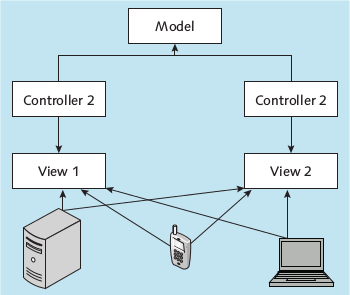
\includegraphics[width=0.7\linewidth]{images/mvc_arch.png}
		\captionof{figure}[Model-View-Controller-Architekturmuster]{Model-View-Controller-Architekturmuster\cite[S.123]{AntoEinf2014}}
		\label{fig:mvcarch}
	\end{minipage}

Durch diese Trennung können z. B. zwei verschiedene Endgeräte das gleiche Model verwenden; der View wird z. B. einmal für die Desktop-Anwendung und einmal für das mobile Endgerät implementiert.\grqq{}\cite[S.123]{AntoEinf2014}

\paragraph{Model}

\paragraph{View}

\paragraph{Controller}
// Vergleich\\

//Abbildung \ref{fig:mvcarch}\\
	\vspace{1em}
	\begin{minipage}{\linewidth}
		\centering
		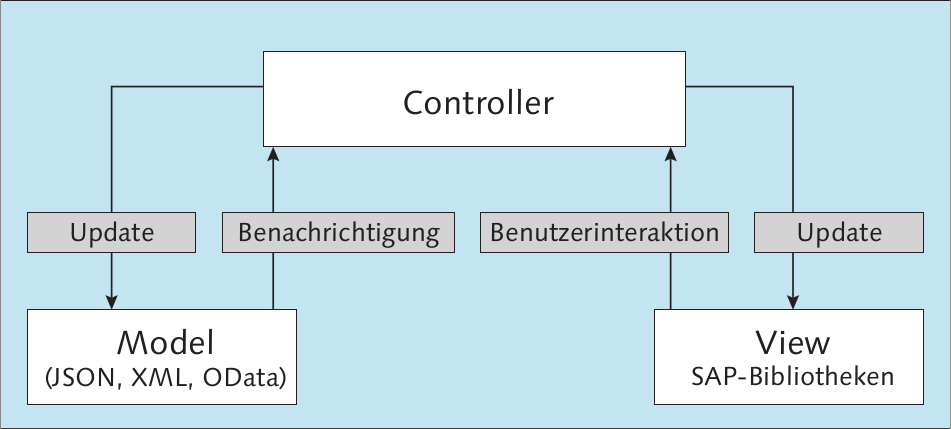
\includegraphics[width=0.7\linewidth]{images/mvc_arch2.png}
		\captionof{figure}[Model-View-Controller-Architekturmuster]{MVC-Architekturmuster\cite[S.124]{AntoEinf2014}}
		\label{fig:mvcarch}
	\end{minipage}

\subsubsection{OData Protokoll}
\glqq Das Open Data Protocol (OData) ist ein von Microsoft veröffentlichtes Protokoll. Das Protokoll basiert auf HTTP und baut auf den älteren Protokollen \ac{ODBC} und \ac{JDBC} auf. OData ist primär für die sogenannten CRUD-Operationen, (Create, Read, Update und Delete) implementiert worden.\grqq{}\cite[S.168]{AntoEinf2014}

// SAP Netweaver Gateway OData Services\\
\pagebreak

% ----------------------------------------------------------------------------------------------------------
% Kapitel
% ----------------------------------------------------------------------------------------------------------
\section{Software Ergonomie}
// Beleg für die Wichtigkeit von Software Ergonomie\\
// Kurze Übersicht über das Themenfeld Software Ergonomie\\
// Wichtigsten Aspekte nennen und näher erläutern\\

\subsection{Definition}
\paragraph{Kognitionspsychologie}
// Modellierung und Simulation von menschlichen Denk- und Wahrnehmungsprozessen\\

\paragraph{Arbeitsphysiologie, Industrieanthropologie}
// Beschäftigung mit grundlegenden menschlichen Fähigkeiten zur Informationsaufnahme und Informationsverarbeitung\\

\paragraph{Arbeitspsychologie}
// Untersuchung der Wechselbeziehungen zwischen Arbeit, deren Schnittstellen und psychischen Faktoren (unter anderem Arbeitszufriedenheit und -unlust)\\

\subsection{DIN EN ISO 9241}
// DIN Norm zur Software Ergonomie\\
// Die 7 Grundsätze der Dialoggestaltung:
\begin{compactitem}
	\item Aufgabenangemessenheit
	\item Selbstbeschreibungsfähigkeit
	\item Erwartungskonformität
	\item Fehlertoleranz
	\item Steuerbarkeit
	\item Individualisierbarkeit
	\item Lernförderlichkeit
\end{compactitem}
\paragraph{DIN EN ISO 14915}
$\;$ \\
// Erweiterung der ISO 9241\\

\subsection{Analyse Methoden}
\paragraph{Eye Tracking}
// Funktionsweise und Ergebnis\\

\paragraph{Mouse Clicking}
// Funktionsweise und Ergebnis\\

\subsection{SAP Technologien in Bezug auf Software Ergonomie}
\subsubsection{Business Server Pages}
// \ac{BSP} ist old school Technik\\
// geklaut von \ac{JSP}\\

\subsubsection{Web Dynpro for ABAP}
// Aktuelle Technik\\
// ABAP Code generiert HTML\\
// statischer und dynamischer Teil\\

\subsubsection{SAP Fiori / SAP UI5 / SAP Screen Personas}
// cutting edge\\
// aktuelle SAP UI Strategie\\
// SAP Präsi Chart Fiori/SP renew, etc. pp\\
// SAP Fiori einerseits Name des Themes/Guideline\\
// andererseits Bündel der gängigsten TAs/GPs als fertige\\
// Mobile First/Responsive Design Applikationen\\
// SAP UI5 - SAPs Framework zur Entwicklung von eigenen Applikationen im Fiori Style\\
// Nicht zu tief auf JS, HTML etc eingehen, dass kommt im nächsten Kapitel\\
// SAP SP - Zusätzliche Schicht um Standard Dynpro zu Personalisieren und so\\
\pagebreak

% ----------------------------------------------------------------------------------------------------------
% Kapitel
% ----------------------------------------------------------------------------------------------------------
\section{Fallbeispiel SAP UI5}
Lorem ipsum dolor sit amet.

\subsection{Beschreibung}
// Frontend - Browser, Elemente\\
// Backend - JSON, OData Model\\
// Analyse der wichtigen Arbeitsschritte\\

\subsection{Hilfsmittel}
\subsubsection{Entwicklungsumgebung}
\paragraph{Eclipse} Zum Einsatz in der Implementierung des Fallbeispiels ist die quelloffene integrierte Entwicklungsumgebung Eclipse gekommen. Diese \ac{IDE} wurde von der Eclipse Foundation entwickelt und ist plattformunabhängig. Geschrieben wurde Eclipse in Java. Die aktuelle Version 4.4 ist am 25. Juni 2014 erschienen und trägt den Namen Luna. Eclipse zeichnet sich durch ein Plugin System aus mit welchem eine erhebliche Anzahl an Anwendungsfälle mit dieser IDE abgedeckt werden können.(vgl. \cite{WikiEclipse2014}) So auch die Entwicklung von SAP UI5 Applikationen. Dafür hat die SAP AG ein spezielles SAP UI5 Plugin bereitgestellt. Entsprechende Plugins müssen nicht umständlich über eine Webseite bezogen und installiert werden. Sie können über die integrierte Plugin Funktion installiert und eingerichtet werden. Eine URL zum Plugin ist vollkommen ausreichend. Für die Entwicklung von SAP UI5 Applikationen wurden folgende Plugins benötigt:

    \begin{compactitem}
	    \item UI Development Toolkit for HTML5
	    \item ABAP Development Tools for SAP NetWeaver
	    \item (SAP HANA Tools)	    
    \end{compactitem}

Bezogen werden können diese Plugins mittels der URL \textit{https://tools.hana.ondemand.com/luna} und der erwähnten Plugin Funktion von Eclipse. Neben dem reinen Code Editor werden allerdings weitere Tools benötigt um eine SAP UI5 Applikation zu entwickeln.

\paragraph{Chrome Developer Tools}
Die SAP UI5 Dokumentation schlägt vor zum Testen der entwickelten Applikationen Google Chrome oder Mozilla Firefox anstatt Microsoft Internet Explorer zu verwenden. Das vorliegende Fallbeispiel wurde mit Google Chrome getestet. Google Chrome bietet dazu ein Tool mit dem Namen Developer Tools, welches in jeder Standard Installation des Browsers enthalten ist. Mit diesem Tool lässt sich beispielsweise das DOM der aktuellen Webseite anzeigen. Weiter kann man JavaScript Breakpoints setzen und so effizient debuggen. Es bietet eine Konsole um direkte JavaScript Befehle abzusetzen und die Ergebnisse zu analysieren. Um eine Anwendungen nicht zwingend auf verschiedenen Endgeräten, mit verschiedenen Displaygrößen, testen zu müssen lassen sich jegliche Art von Endgeräten mit den Developer Tools emulieren.(vgl. \cite{DevTools})

\paragraph{Neptune Application Designer}


\subsubsection{UI Design und Prototyping}
// Wireframing als Prototyping\\
// Abbildung Wireframesketcher\\

\subsection{Implementierung}
\subsubsection{View}
// Auszugsweise Coding bringen um bestimmte Elemente aus der Theorie zu zeigen\\
// Generellen Aufbau der Views erklären\\
// Kapselung wird dadurch verdeutlicht\\
// Listing \ref{lst:app.view.js}
	\vspace{1em}
	\begin{lstlisting}[caption=Root View der Applikation, label=lst:app.view.js]
sap.ui.jsview("abat.Mockup.view.App", {

  getControllerName: function () {
    return "abat.Mockup.view.App";
  },
  
  createContent: function (oController) {
    // to avoid scroll bars on desktop
    this.setDisplayBlock(true);
    
    // create app
    this.app = new sap.m.SplitApp();
    
    // load the master page
    var master = sap.ui.xmlview("Master", "abat.Mockup.view.Master");
    master.getController().nav = this.getController();
    this.app.addPage(master, true);
    
    // load the empty page
    var empty = sap.ui.xmlview("Empty", "abat.Mockup.view.Empty");
    this.app.addPage(empty, false);
    
    // wrap app with shell
    return new sap.m.Shell("Shell", {
      title : "{i18n>ShellTitle}",
      showLogout : false,
      app : this.app
    });
  }
});
	\end{lstlisting}

// Master/Detail Applikation mit Fragment und Chart View Aufbau\\
// TODO: Visio Diagramm oder vergleichbares erstellen\\
// sap.ui.view\\
//   |- sap.m.Shell\\
//   |  |- sap.m.SplitApp\\
//   |  |  |- sap.m.Page\\
//   |  |  |  |- sap.m.Bar\\
//   |  |  |  |- sap.m.Bar\\
//   |  |  |  |- sap.m.List\\
//   |  |  |  |  |- sap.m.ObjectListItem\\
//   |  |  |  |- sap.m.Bar\\
//   |  |  |- sap.m.Page\\
//   |  |  |  |- sap.m.ObjectHeader\\
//   |  |  |  |  |- sap.m.ObjectAttribute\\
//   |  |  |  |  |- sap.m.ObjectAttribute\\
//   |  |  |  |  |- sap.m.ObjectAttribute\\
//   |  |  |  |  |- sap.m.ObjectAttribute\\
//   |  |  |  |  |- sap.m.ObjectStatus\\
//   |  |  |  |- sap.IconTabBar\\
//   |  |  |  |  |- sap.IconTabFilter\\
//   |  |  |  |  |  |- sap.ui.core.Fragment\\
//   |  |  |  |  |  |  |- sap.ui.core.FragmentDefinition\\
//   |  |  |  |  |  |  |  |- sap.viz.ui5.Bar\\
//   |  |  |  |  |- sap.IconTabFilter\\
//   |  |  |  |  |  |- sap.ui.core.Fragment\\
//   |  |  |  |  |  |  |- sap.ui.core.FragmentDefinition\\
//   |  |  |  |  |  |  |  |- sap.viz.ui5.Bar\\
//   |  |  |  |- sap.m.Bar\\


\subsubsection{Model und Controller}
// die Verbindung von beiden Anhand von Coding zeigen\\
// TODO: OData Modell einbinden\\
// Listing \ref{lst:Component.js}
	\vspace{1em}
	\begin{lstlisting}[caption=Component.js - Datenmodell an die Root View binden, label=lst:Component.js]
...
// JSON Modell an die Root View binden
var oModel = new sap.ui.model.json.JSONModel("model/mock.json");
oView.setModel(oModel);

// OData Modell
var oModel = new sap.ui.model.odata.ODataModel(<URL>);
oView.setModel(oModel);

// I18N(Lokalisierung) Modell
var i18nModel = new sap.ui.model.resource.ResourceModel({
  bundleUrl : "i18n/messageBundle.properties"
});
oView.setModel(i18nModel, "i18n");

// Geraetespezifisches Modell
var deviceModel = new sap.ui.model.json.JSONModel({
  isPhone : jQuery.device.is.phone,
  listMode : (jQuery.device.is.phone) ? "None" : "SingleSelectMaster",
  listItemType : (jQuery.device.is.phone) ? "Active" : "Inactive"
});
deviceModel.setDefaultBindingMode("OneWay");
oView.setModel(deviceModel, "device");
...
	\end{lstlisting}

\subsubsection{Backend}
// ABAP Stack der den RESTful Service bereitstellt zeigen\\
// Beispielhafte Implementation des HTTP Responses\\
\pagebreak

% ----------------------------------------------------------------------------------------------------------
% Kapitel
% ----------------------------------------------------------------------------------------------------------
\section{Analyse}
\subsection{Heatmap}
// Angewandte Analyse mit Heatmap\\

\subsection{UI-Objekte}
// Mobile First/Responsive Design\\

\subsection{PLATZHALTER}
// PLATZHALTER\\
\pagebreak

% ----------------------------------------------------------------------------------------------------------
% Kapitel
% ----------------------------------------------------------------------------------------------------------
\section{Schluss}
Lorem ipsum dolor sit amet.

\paragraph{Zusammenfassung}
// Arbeitsgebiete, Produktions \& Dienstleistungsbereiche\\
// Arbeitsergebnisse\\
// Projektziele, Projektergebnisse, Projekttermine\\
// Mitwirkungszeiträume\\
// Liste aller selbst wahrgenommen Aufgaben und Tätigkeiten\\
// Projektmeilensteine\\
// Ablauforganisation \& Beteiligte\\
// Arbeitsformen, Arbeitsmittel, Arbeitsabläufe\\
// Kommunikations- / Informationsgewohnheiten\\
// Auswertung relevanter Literatur\\
// Themen aus Lehrveranstaltungen\\

\paragraph{Bewertung}
// Wesentliche Erkenntnisse und Erfahrungen\\
// Folgerungen und Konsequenzen\\
// Vorschläge für Verbesserung und Veränderung\\
// Auswirkungen auf persönliche Berufs- und Karriereplanung\\
// Bezug zum Studium\\
// hilfreiche Studieninhalte\\
// neu gewonnenes Interesse\\
\pagebreak

% ----------------------------------------------------------------------------------------------------------
% Literatur
% ----------------------------------------------------------------------------------------------------------
\renewcommand\refname{Quellenverzeichnis}
\bibliographystyle{myalpha}
\bibliography{bibo}
\pagebreak

% ----------------------------------------------------------------------------------------------------------
% Anhang
% ----------------------------------------------------------------------------------------------------------
\pagenumbering{Roman}
\setcounter{page}{1}
\lhead{Anhang \thesection}

\begin{appendix}
\section*{Anhang}
\phantomsection
\addcontentsline{toc}{section}{Anhang}
\addtocontents{toc}{\vspace{-0.5em}}

\section{GUI}
Ein toller Anhang.

\subsection*{Screenshot}
\label{app:screenshot}
Unterkategorie, die nicht im Inhaltsverzeichnis auftaucht.

\end{appendix}

\newpage
\thispagestyle{empty}
\begin{center}
	\vspace*{5em}
	\huge\textbf{Erklärung}\\
\end{center}
\vspace{2em}
Hiermit versichere ich, dass ich meine Abschlussarbeit selbständig verfasst und keine anderen als die angegebenen Quellen und Hilfsmittel benutzt habe.

\vspace{4em}
\begin{minipage}{\linewidth}
	\begin{tabular}{p{15em}p{15em}}
		Datum: &  .......................................................\\
		& \centering (Unterschrift)\\
	\end{tabular}
\end{minipage}

\end{document}
